\section{Anpassung der existierenden Lösung}
Infrastrukturelle Anpassungen wurden im Buildsystem vorgenommen. Herausfordernd war das initiale Setup des bestehenden Projekts, da hierfür die Installation von externen Abhängigkeiten notwendig ist. Außerdem müssen Dateistrukturänderugen in der Builddatei von CMAKE reflektiert werden. Um die zukünftige Installation auf weiteren Systemen zu vereinfachen, wurde das Buildtool CMAKE angepasst und das Projekt zur Befehlsaggregation mit einer Makefile ergänzt.

\subsection{CMAKE}
\label{sec:cmake}
Wie schon bereits einleitend in Kapitel \ref{sec:buildsystem} erläutert, muss das Buildsystem angepasst werden. Hierfür wurden die CMAKE Files angepasst, sowie die Struktur des Codes. Der vorgegebene Code nutzt absolute Pfade für die Abhängigkeiten. Dies erschwert das Zusammenarbeiten und Aufsetzten des Codes. Das gesamte Buildsystem musste angepasst werden, damit beim Aufsetzten des Repositories nicht noch Pfade in den CMAKE-Dateien angepasst werden müssen. Dafür wurde der package manager VCPKG, als GIT-Submodule zum Repository hinzugefügt. Dadurch wird beim Herunterladen des Repositories auch der package manager mit Installiert und in der CMAKE-Datei kann ein Relativer Pfad angegeben werden. Damit VCPKG installiert wird und die benötigten Abhängigkeiten installiert werden, wurde zusätzlich eine Makefile hinzugefügt. Mittels dieser kann VCPKG durch einen Make-Befehl installiert werden und durch einen Zweiten Make-Befehl alle Abhängigkeiten (nlohmann-json, mlpack, gRPC) installiert. Durch das verwenden des VCPKG package manager können die Abhängigkeiten durch die CMAKE-Befehle \textit{find\_package} und \textit{find\_path} eingebunden werden und es benötigt keine Anpassungen der Pfade.

\subsection{Makefile}
Um das Projekt zu kompilieren, mussten manuell viele Parameter manuell angepasst werden. Zum Beispiel musste der Pfad zum \verb|vcpkg| in einem CMakeLists-File angepasst werden. Um solche umständlichen und nicht ganz trivialen Schritte zu vereinfachen, wurde das Makefile erstellt. Dieses ist in Listing \ref{code:Makefile} dargestellt.\\

\begin{lstlisting}[caption=Makefile, label={code:Makefile}, captionpos=b]
    .PHONY: about init install-dependencies build compile start-subscale start-server start-client kill-server clean

    VCPKG_DIR := ./include/vcpkg
    VCPKG := ./include/vcpkg/vcpkg
    
    about:
	    @echo "Makefile to help manage subscale gpu project"
	    @echo "commands:"
	    @echo "     - init: make sure vcpkg ist cloned as submodule"
	    @echo "     - install-dependencies: install all vcpkg dependencies"
	    @echo "     - build: build cmake changes"
	    @echo "     - compile: compile the code"
	    @echo "     - start-subscale: start subscale local"
	    @echo "     - start-server: starts a server to which the client sends data to   calculate"
	    @echo "                     default port is 8080, else set with     -p=<port-number>"
	    @echo "     - start-client: starts execution subscale distributed"
	    @echo "     - kill-server: kills all servers still running in background"
	    @echo "     - removes builded files"
    
    init:
        git submodule update --init --recursive && $(VCPKG_DIR)/bootstrap-vcpkg.sh && mkdir Proto/generated
    
    install-dependencies:
        $(VCPKG) install nlohmann-json && $(VCPKG) install mlpack && $(VCPKG) install grpc
    
    build:
        cmake -S . -B ./debug
    
    compile:
        cmake --build ./debug
    
    start-subscale:
        ./debug/Subscale/subscale
    
    start-server:
        ./debug/Server/server $(p)
    
    start-client:
        ./debug/Client/client
    
    kill-server:
        killall ./debug/Server/server
    
    clean:
        rm -rf ./debug
\end{lstlisting}

Durch die Verwendung dieser Makefile-Befehle soll es vereinfacht werden, den Code zum einen manuell in seiner eignen Umgebung ausführen zu können, als auch zum anderen automatisiert innerhalb eines Docker-Containers.

Da das \verb|vcpkg| als Submodule integriert wurde, was die automatisierte Installation und Pfadfindung von \verb|vcpkg| als auch \verb|gRPC|, \verb|mlpack| und \verb|nlohmann-json| ermöglicht, können alle benötigten Schritte per \verb|make init| (Zeilen 20f) und \verb|make install-dependencies| (Zeilen 23f) sehr einfach und automatisiert installiert und integriert werden. Es besteht weiterhin die Möglichkeit in den CMakeLists-Files dies manuell anzupassen und diese beiden Makefile-Befehle zu ignorieren. Dies ist sinnvoll, wenn man Docker-Container besitzt, welche dies im Vorhinein bereits installiert haben oder man das \verb|vckpg| aus seiner eigenen Entwicklungsumgebung nutzen möchte.

Um das Projekt an sich über CMAKE zu bauen, wird dies durch \verb|make build| (Zeilen 26f) vereinfacht. Das Kompilieren des Codes wird auch durch das Makefile unterstützt. Dazu kann mit \verb|make compile| (Zeilen 29f) der Code kompiliert werden.

Wenn man den Subscale-Algorithmus starten möchte, bietet das Makefile ebenfalls Möglichkeiten, dies vereinfacht zu tun. So kann mit \verb|make start-subscale| (Zeilen 32f) die lokale Ausführung auf einem Rechner gestartet werden. Über \verb|make start-server| (Zeilen 35f) beziehungsweise \verb|make start-client| (Zeilen 38f) kann der Server beziehungsweise Client für die verteilte Ausführung gestartet werden. Wenn man den Server startet, hat man die Möglichkeit den Port, über welchen dieser gestartet werden soll, zu setzten. So kann man mit \verb|make start-server -p=8080| sagen, dass der Server auf den Port 8080 hören soll.

Falls man einen Server richtig beenden möchte, weil dieser aus unerklärlichen Gründen weiterhin im Hintergrund läuft, kann man dies auch über den Befehl \verb|make kill-server| tun und erspart sich die manuelle PID-Findung.

Zuletzt kann auch alles, was durch das Projekt gebaut wurde, wieder mit \verb|make clean| (Zeilen 44f) entfernt werden.

\subsection{Umstrukturierung}
Der Vorgegebene Code war nicht dafür ausgelegt diesen zu verteilen, deshalb muss die Struktur angepasst werden. Dies ist vor allem auch notwendig damit unabhängig voneinander gearbeitet werden kann ohne das Merge-Konflikte entstehen. Der Vorgegebene Code hatte folgende Struktur:
\dirtree{%
.1 data.
.1 packages.
.1 SubscaleGPU.
.2 ....
.1 CMakeLists.txt.
.1 config.json.
}
Der Komplette Subscale-Algorithmus befand sich in dem Ordner \textit{SubscaleGPU}, die dazugehörigen Daten in dem \textit{data} Ordner. Zusätzlich benötigte Libraries befanden sich im \textit{packages} Ordner. Die Aktuelle Struktur erschwerte das hinzufügen einer Client-Server-Architektur. Der Code muss umstrukturiert werden, damit gleichzeitig an Client, Server und dem Subscale-Algorithmus gearbeitet werden kann. Der Komplette Subscale Algorithmus wurde in einen eigenen Ordner verschoben und als Statische Library weiterentwickelt, somit kann dieser einfach im Client und Server eingebunden werden. Des Weiteren benötigt sowohl Client als auch Server die Protobuf-Dateien, dafür wurden die .proto-Dateien in einen eigenen Ordner gelegt und von Client und Server verwendet zum Entwickeln der Schnittstellen. Die daraus entstandene Struktur sieht folgendermaßen aus:

\dirtree{%
.1 Client.
.1 include.
.2 vcpkg.
.1 Proto.
.2 subscale.proto.
.1 Server.
.1 SubscaleGPU.
.2 data.
.2 Config.
.1 CMakeLists.txt.
}

\subsection{Aufbau des originalem Code}
Der originale Code hatte eine Klasse \emph{LocalSubspaceTable}, die für das Darstellen der \emph{Subspace}-Tabelle zuständig war.
Diese Klasse wurde sowohl für die \emph{Slices} als auch für die gesamten \emph{Subspaces} verwendet. Meine Idee war es dann,
den anderen im Team eine Funktion names \emph{calculateRemote} bereitzustellen, die als Parameter die \emph{Labels}, den \emph{minBound} des Slices und den 
\emph{maxBound} des Slices bekommt und den berechneten Slice als Form der \emph{LocalSubspaceTable}-Klasse zurückgibt.

Im Folgenden wird zunächst der Aufbau des originalen Code erläutert, um anschließend die Umsetzung der \emph{calculateRemote}-Methode
von unten nach oben darzustellen.\\
Der Code bestand im wesentlichen aus einer abstrakten Klasse \emph{ISubscale} und zwei konkreten Implementierungen
\emph{Subscale} (\emph{Cuda}-Implementation) und \emph{SubscaleSec} (normale Implementation) wie im folgenden gezeigt:
\newpage
\begin{figure}[h]
    \centering
    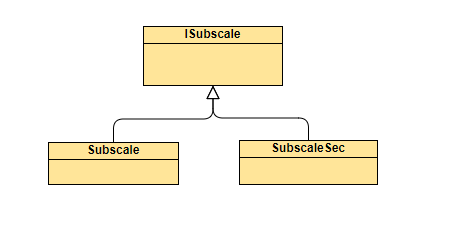
\includegraphics[width=\textwidth]{Subscale.png}
    \caption{Subscale}
    \label{img:subscale}
\end{figure}

\emph{ISubscale} selber hatte eine Funktion \emph{calculateClusterCandidates} die Vorbereitungen getroffen hat und die 
konkrete Implementierung sollte die Funktion \emph{calculateAllSlices} überschreiben, die den Zweck hatte, alle \emph{Slices}
zu erstellen und auf die Festplatte zu schreiben. Außerdem verfügte \emph{ISubscale} noch über eine Funktion \emph{combineAllSlices}
die die einzelnen Slices von der Festplatte geholt hat, die Slice verengert hat und dann zu der endgültigen Subspace Tabelle 
hinzugefügt hat.   

\subsection{calculateSlice}
Angefangen am untersten Ende brauchten die beiden konkreten Implementationen eine neue Funktion, die alle nötigen Informationen 
bekommt, um einen Slice zu erstellen und als Rückgabe dann den Slice zurückgibt. Da sich die konkreten Implementationen nur in der 
Erzeugung der konkreten Klassen unterscheidet, wird in dieser Section der generelle Code gezeigt und in den folgenden Abschnitten 
nur die wesentlichen Unterschiede.  

\lstinputlisting[language=C++,caption={calculateSlice},
    label=lst:calculateSlice]{src/calculateSlice.cpp}

Wie in Listing \ref{lst:calculateSlice} zu sehen ist, werden die Berechungsklassen initialisiert und anschließend werden die 
\emph{DenseUnits} erzeugt, um diese dann in eine Subspace Tabelle hinzuzufügen. Sollte der \emph{Slice} nicht leer sein, dann 
werden die Einträge noch nach den Subspaces zusammengefügt. Als letztes wird noch der Speicher von der Grafikkarte zum Host kopiert 
(ist bei der sequentiellen Abarbeitung nicht nötig). 

\subsection{calculateSlice Sequentiell}
In dieser Sektion werden noch die spezifischen Erzeugungen der Berechungsklassen für die Sequentielle Abarbeitung gezeigt.

\lstinputlisting[language=C++,caption={calculateSlice Sequentiell},
    label=lst:calculateSliceSeq]{src/calculateSliceSeq.cpp}

\subsection{calculateSlice Cuda}
In dieser Sektion werden noch die spezifischen Erzeugungen der Berechungsklassen für die \emph{Cuda} Abarbeitung gezeigt.

\lstinputlisting[language=C++,caption={calculateSlice Cuda},
    label=lst:calculateSliceCuda]{src/calculateSliceCuda.cpp}

\subsection{calculateClusterCandidatesRemote}
Die nächst obere Stufe war die \emph{calculateClusterCandidatesRemote}-Methode, die alle notwendigen 
Informationen für die \emph{calculateSlice} vorbereitet. Diese sieht wie folgt aus:

\lstinputlisting[language=C++,caption={calculateClusterCandidatesRemote},
    label=lst:calculateClusterCandidatesRemote]{src/calculateClusterCandidatesRemote.cpp}

Diese hat die \emph{CoreSets} erzeugt und die weiteren Informationen weiter runter gegeben.

\subsection{calculateRemote}
Der letzte Schritt war dann, die \emph{calculateRemote}-Methode, die lediglich die \emph{config}
gelesen hat und dann die konkrete Implementierung des \emph{Subscales} erzeugt hat. 

\lstinputlisting[language=C++,caption={calculateRemote},
    label=lst:calculateRemote]{src/calculateRemote.cpp}